\begin{adjustwidth*}{}{-2.25in}
\textbf{{\large Exercises}}
\setlength{\columnsep}{25pt}
\begin{multicols*}{2}
\noindent Terms and Concepts \small
\begin{enumerate}[1)]
\item {T/F: Let $f$ be a position function. The average rate of change on $[a,b]$ is the slope of the line through the points $(a, f(a))$ and $(b,f(b))$.}
\item {T/F: The definition of the derivative of a function at a point involves taking a limit.}
\item {In your own words, explain the difference between the average rate of change and instantaneous rate of change.}
\item Let $y = f(x)$. Give three different notations equivalent to ``$f'(x)$.''
\end{enumerate} 

\noindent {\normalsize Problems} \small

\noindent {\bf In exercises 5--8, a graph of a function is given. Using the graph, sketch $f'(x)$.}

\begin{enumerate}[1),resume]
\item 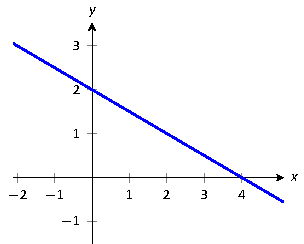
\includegraphics[scale=.8]{figures/fig02_01_ex_26}
\item 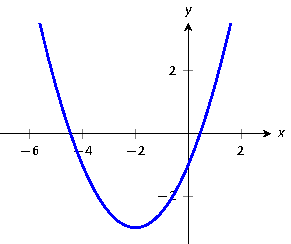
\includegraphics[scale=.8]{figures/fig02_01_ex_27}
\item 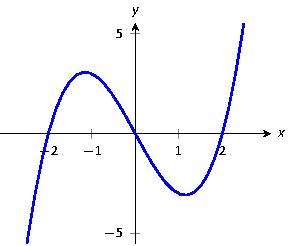
\includegraphics[scale=.8]{figures/fig02_01_ex_28}
\item 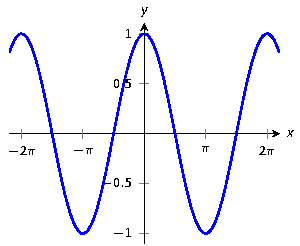
\includegraphics[scale=.8]{figures/fig02_01_ex_29}

\item Using the graph of $g(x)$ below, answer the following questions.
\ba
\item Where is $g(x) > 0$?
\item Where is $g(x) < 0$?
\item Where is $g(x) = 0$?
\item Where is $g'(x) < 0$?
\item Where is $g'(x) > 0$?
\item Where is $g'(x) = 0$?
\ea

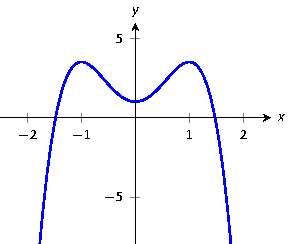
\includegraphics[scale=.8]{figures/fig02_01_ex_30}

\item Let $f$ be a function with the following properties:  $f$ is differentiable at every value of $x$ (that is, $f$ has a derivative at every point), $f(-2) = 1$, and $f'(-2) = -2$, $f'(-1) = -1$, $f'(0) = 0$, $f'(1) = 1$, and $f'(2) = 2$.
\ba
	\item On the axes provided at left below, sketch a possible graph of $y = f(x)$.  Explain why your graph meets the stated criteria.
	\item On the axes at right below, sketch a possible graph of $y = f'(x)$.  What type of curve does the provided data suggest for the graph of $y = f'(x)$?
	\item Conjecture a formula for the function $y = f(x)$.  Use the limit definition of the derivative to determine the corresponding formula for $y = f'(x)$.  Discuss both graphical and algebraic evidence for whether or not your conjecture is correct.
\ea

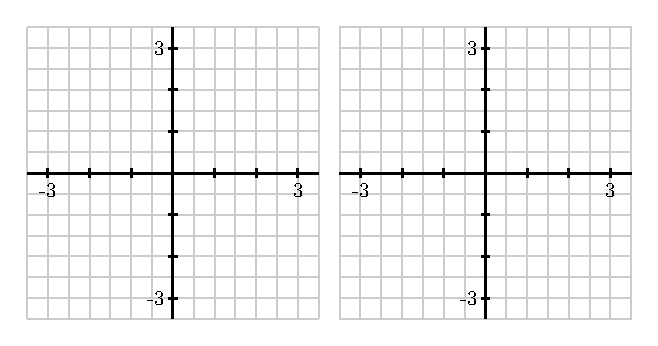
\includegraphics[scale=.75]{figures/1_2_Ez3.eps} 
\end{enumerate}

%------------------------------------------
% END OF EXERCISES ON FIRST PAGE
%------------------------------------------
\end{multicols*}
\end{adjustwidth*}

\clearpage

\begin{adjustwidth*}{}{-2.25in}
\setlength{\columnsep}{25pt}
\begin{multicols*}{2}\small

\begin{enumerate}[1),start=11]
\item Let $g$ be a continuous function (that is, one with no jumps or holes in the graph) and suppose that a graph of $y= g'(x)$ is given by the graph on the right below.

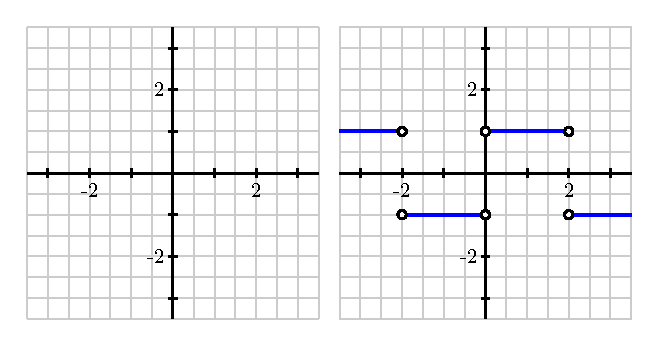
\includegraphics[scale=.75]{figures/1_4_Ez2.eps} %\ \  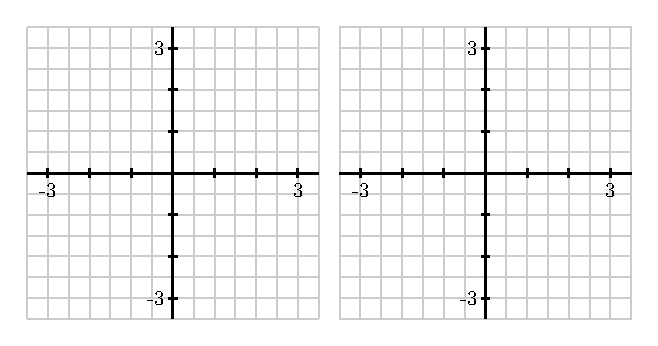
\includegraphics{figures/1_2_Ez3.eps}

\ba
\item Observe that for every value of $x$ that satisfies $0 < x < 2$, the value of $g'(x)$ is constant.  What does this tell you about the behavior of the graph of $y = g(x)$ on this interval?
\item On what intervals other than $0 < x < 2$ do you expect $y = g(x)$ to be a linear function?  Why?
\item At which values of $x$ is $g'(x)$ not defined?  What behavior does this lead you to expect to see in the graph of $y=g(x)$?
\item Suppose that $g(0) = 1$.  On the axes provided at left, sketch an accurate graph of $y = g(x)$.
\ea

\item Consider the graph of the function $y = p(x)$ that is provided below on the left.  Assume that each portion of the graph of $p$ is a straight line, as pictured.

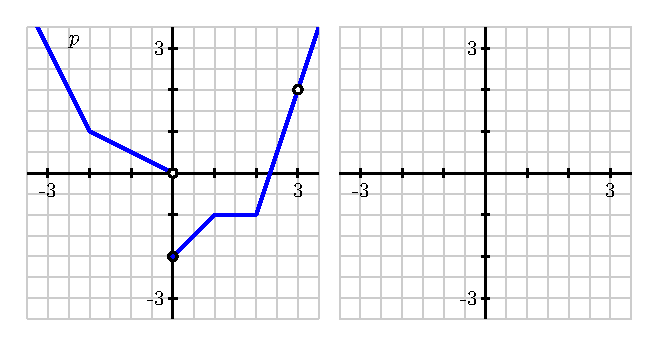
\includegraphics[scale=.75]{figures/1_7_Ez2.eps}

\ba
\item State all values of $a$ for which $\lim_{x \to a} p(x)$ does not exist.
\item State all values of $a$ for which $p$ is not continuous at $a$.
\item State all values of $a$ for which $p$ is not differentiable at $x = a$.
\item On the axes provided on the right, sketch an accurate graph of $y = p'(x)$.
\ea

\item For each of the following prompts, give an example of a function that satisfies the stated criteria.  A formula or a graph, with reasoning, is sufficient for each.  If no such example is possible, explain why.
\ba
\item A function $f$ that is continuous at $a = 2$ but not differentiable at $a = 2$.
\item A function $g$ that is differentiable at $a = 3$ but does not have a limit at $a=3$.
\item A function $h$ that has a limit at $a = -2$, is defined at $a = -2$, but is not continuous at $a = -2$.
\item A function $p$ that satisfies all of the following:
\begin{itemize}
\item $p(-1) = 3$ and $\ds\lim_{x \to -1} p(x) = 2$
\item $p(0) = 1$ and $p'(0) = 0$
\item $\ds\lim_{x \to 1} p(x) = p(1)$ and $p'(1)$ does not exist
\end{itemize}
\ea
\end{enumerate}

\vspace{.25cm}

\noindent {\bf For exercises 14--22, use the limit definition of the derivative to compute the derivative function.}

\bmtwo
\begin{enumerate}[1),resume]
\item $\ds f(x) = 8x$
\item $\ds y = x^2$
\item $\ds g(x) = 2x^2 + 3x$
\item $\ds s(t) = \frac{1}{\ds \sqrt{t}}$
\item $\ds r(x) = \frac{1}{x^2}$
\item $\ds f(x) = \ds\sqrt{3x-1}$
\item $\ds f(x) = \ds\sqrt{8x}$
\item $\ds s(t) = \frac{1}{t + 5}$
\item $\ds y = \frac{1}{2x - 1}$
\end{enumerate}
\emtwo

%------------------------------------------------
% END OF EXERCISES ON SECOND PAGE
%------------------------------------------------
\end{multicols*}
\end{adjustwidth*}
\afterexercises